
\documentclass[10pt]{beamer}

\usetheme[progressbar=frametitle]{metropolis}% modern fork of the metropolis theme
\usepackage[natbib=true,backend=biber,useprefix=true,sorting=none]{biblatex}
\addbibresource{referencias.bib}

\usepackage{booktabs}
\usepackage[scale=2]{ccicons}

\usepackage{pgfplots}
\usepgfplotslibrary{dateplot}

\usepackage{outlines}
\usepackage[spanish]{babel} % Idioma español

\usepackage{xspace}
\newcommand{\themename}{\textbf{\textsc{metropolis}}\xspace}
\renewcommand*{\bibfont}{\normalfont\small}

\title{\small Proyecto de tesis de maestría}
\subtitle{\textbf{\large Identificación de potencial sesgo por no respuesta\\
\large en encuestas de hogares del nordeste argentino \\ 
\large sobre el ingreso familiar y el nivel de pobreza}}

\date{\scriptsize Diciembre 2024}

\author{
\noindent\begin{tabular}{@{}ll}
    Tesista & Lic. Celine Iliana Cabás\\
    Directora &  Dra. Patricia Caro\\
    Co-Director & Dr. Carlos Matías Hisgen
    \end{tabular}
    \\
    \\
}

\institute{
    Maestría en Estadística Aplicada \\
    Universidad Nacional de Córdoba}

\titlegraphic{\hfill
\includegraphics[height=1cm]{unc3_e.jpg}}

\begin{document}

\maketitle

\begin{frame}{Contenidos}
  \setbeamertemplate{section in toc}[sections numbered]
  \tableofcontents[hideallsubsections]
\end{frame}

\section{Introducción}

\begin{frame}[fragile]{Introducción}

\begin{quote}
"Si la decisión de responder depende estadísticamente de las variables bajo investigación, entonces la submuestra de encuestados no reflejará con precisión la distribución real de las variables de interés en la población y esto, a su vez, dará como resultado inferencias basadas en muestras sistemáticamente sesgadas". \cite{korinek07}
\end{quote}

\begin{itemize}
    \item No respuesta en encuestas de hogares.
    \item Caso particular: Encuesta Permanente de Hogares (EPH).
    \item Producto estadístico utilizado para medir distribuciones de ingresos y nivel de pobreza por aglomerado urbano.
    \item Cobertura geográfica: Nordeste Argentino.
\end{itemize}

\end{frame}

\begin{frame}{¿Qué ocurre en el NEA?}
  \begin{figure}
      \centering
      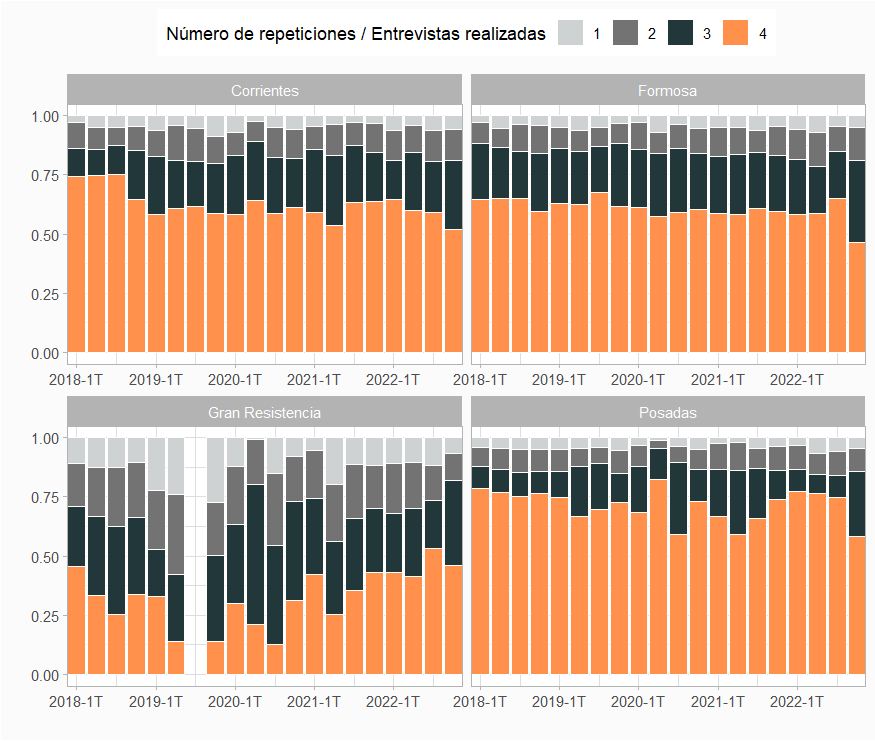
\includegraphics[width=0.75\linewidth]{Rplot01.png}
      \caption{Estructura de respuesta por aglomerado urbano, 2018-2022.}
      \label{fig:enter-label}
  \end{figure}
\end{frame}

\begin{frame}[fragile]{Introducción}

\begin{itemize}
    \item ¿Qué ocurriría si la estructura de respuesta depende del ingreso?
    \item ¿De qué manera puede equilibrarse la representatividad de los hogares en la muestra? ¿Cómo mejorar la representatividad de quienes tienden a no responder?
    \item La selección del NEA viene justificada por el interés de estudiar si las diferencias entre el nivel de pobreza monetaria de Gran Resistencia y los demás aglomerados urbanos de la región puede verse justificada por diferencias observables en sus estructuras de no respuesta.
\end{itemize}

\end{frame}

\section{Antecedentes}

\begin{frame}[fragile]{Marco teórico I}

\rightarrow \textbf{¿Qué entendemos por no respuesta?} 

No respuesta al ítem o \textit{no respuesta unitaria} \cite{korinek07}


\rightarrow \textbf{¿Cuándo existe sesgo por no respuesta?} 

Cuando las personas que sí respondieron a la encuesta difieren significativamente de aquellas que no lo hicieron, es decir, la no respuesta \textit{no se comporta de manera aleatoria} \cite{wmethods}.

\rightarrow \textbf{¿Cómo detectar el sesgo por no respuesta?}

\begin{itemize}
    \item Test de Little \cite{tesisgonz};
    \item Test Chi-cuadrado de contraste de independencia \cite{handbook};
    \item Modelos logísticos de respuesta binaria o politómica \cite{handbook}
\end{itemize}

\end{frame}

\begin{frame}[fragile]{Marco teórico II}

\rightarrow \textbf{¿Cómo lidiar con el sesgo? ¿De qué manera corregirlo?}

\begin{outline}
    \1 Técnicas de imputación para sustituir individuos no encuestados. Métodos de calibración basados en variables auxiliares que deben conocerse en la población \cite{handbook} \cite{psa_calib_onlinesv};
    \1\textbf{ Propensity Score Adjustment (PSA)}. Modelos de estimación de la probabilidad de respuesta (propensión a responder):
    \2 Modelos logísticos de respuesta binaria; 
    \2 Modelos multinomiales de respuesta politómica ordinal; 
    \2 Modelos de aprendizaje automático (CART, RF, XGBoost) \cite{methodsml}.
    \1 Recalibrar los pesos de los hogares mejorando la representatividad en la muestra de aquellos con baja propensión a responder respecto a aquellos con alta propensión a responder.
\end{outline}

\end{frame}

    
\begin{frame}{Antecedentes empíricos}

Algunos trabajos aplicados:
\begin{itemize}
    \item Korinek \cite{korinek07} trabaja con la encuesta Current Population Survey (CPS) de U.S. Census Bureau para analizar la sensibilidad de la distribución acumulada del ingreso frente a ajustes en los factores de expansión basados en la no respuesta unitaria.
    \item \textit{En Argentina}, el trabajo de Comari y Hoszowski \cite{nonresponsearg} estudia el efecto de la no respuesta en la EPH (2005-2011) sobre la estimación de la \textit{tasa de desempleo}. Encuentran que los hogares con mayor número de entrevistas realizadas tienen menores tasas de desempleo.
\end{itemize}

\end{frame}

\begin{frame}{Actualizaciones metodológicas}

En Argentina, el INDEC ha incorporado actualizaciones metodológicas referidas a:

\begin{itemize}
    \item  \textit{Ajustes por probabilidad de respuesta} en el factor de expansión basados en las variables: nivel educativo, edad, cantidad de ocupados y desocupados, régimen de tenencia de la vivienda, entre otras \cite{indecmetod}.
    \item \textit{Ajustes sobre el nivel de ingreso}. La no respuesta fue abordada desde el enfoque de ``no respuesta al ítem'' con correcciones mediante ajustes a los pesos de diseño asignando a los no respondentes el comportamiento de los respondentes por estratos \cite{indecmetod2}.
\end{itemize}

\end{frame}

\section{Formulación del problema y objetivos}

\begin{frame}[fragile]{Formulación del problema}

    \metroset{block=fill}

    \begin{block}{Pregunta de investigación}
        ¿Qué efectos tiene la presencia de sesgo por no respuesta en encuestas de hogares del nordeste argentino sobre la estimación del ingreso familiar y el nivel de pobreza?
    \end{block}

\

    \begin{block}{Objetivo general}
       Identificar la potencial presencia de sesgo por no respuesta en encuestas de hogares del nordeste argentino y sus efectos sobre el ingreso familiar y el nivel de pobreza durante el período 2018-2022.
     \end{block}
\end{frame}

\begin{frame}[fragile]{Objetivos específicos}

\begin{itemize}
    \item Comparar las \alert{estructuras de respuesta} de la encuesta de hogares \alert{entre los aglomerados} urbanos del nordeste argentino para el período 2018-2022.
    \item Comprobar si la \alert{predisposición a responder} por parte de los hogares \alert{depende significativamente del ingreso familiar} u otras variables en los distintos aglomerados urbanos del nordeste argentino.
    \item Comparar \alert{modelos para predecir} la probabilidad de los hogares de responder de manera completa el esquema de entrevistas de la encuesta.
    \item Plantear una \alert{corrección del sesgo por no respuesta} basada en la probabilidad predicha de responder mediante técnicas de reponderación de los datos.
    \item  \alert{Contrastar las distribuciones} de ingresos y el nivel de pobreza estimado antes y después de la corrección por no respuesta.
\end{itemize}

\end{frame}

\section{Fuentes de información}

\begin{frame}{Fuentes de información}

Este proyecto se plantea mediante el uso de las siguientes \textbf{fuentes secundarias} de información relevadas por el Instituto Nacional de Estadísticas y Censos (INDEC) de la República Argentina:

\begin{itemize}
    \item Encuesta Permanente de Hogares (EPH), individual y hogar.
    \item Índice de Precios al Consumidor (IPC) para deflactar ingresos.
    \item Valorización de la Canasta Básica Total (CBT) para la determinación de la condición de pobreza de los hogares.
\end{itemize}

\end{frame}

\begin{frame}{Variables preliminares}

\begin{table}
\centering
\caption{\small Variables preliminares a utilizar en EPH individual y hogar.}

\resizebox{7.5cm}{!}{

\label{tab:my_label}
    \begin{tabular}{|rl|} 
        \hline
        \textbf{Variable} & 
        \textbf{Descripción} \\ 
        \hline

        \textbf{Identificación}&\\
        CODUSU & Código de identificación de la vivienda\\
        NRO\_HOGAR & Código de identificación del hogar \\
        REGION&Código de región geográfica\\
        AGLOMERADO & Código de aglomerado urbano \\
        ANO4&Año de relevamiento\\
        TRIMESTRE&Trimestre de relevamiento\\
        
        \hline
        \textbf{Base individual}&\\
        CH03&Relación de parentesco (Jefe de hogar=1)\\
        CH04&Sexo\\
        CH06&Edad \\
        NIVEL\_ED&Nivel educativo\\
        ESTADO&Condición de actividad\\
        CAT\_OCUP&Categoría ocupacional\\
        
        \hline
        \textbf{Base hogar}&\\
        IV1&Tipo de vivienda\\
        IX\_TOT&Cantidad de miembros del hogar\\
        ITF&Ingreso total familiar\\
        IPCF&Ingreso per cápita familiar\\ 

        \hline
        \textbf{Variable de respuesta}&\\
        NRO\_REP&Número de entrevistas realizadas en el período 2018-2022\\ 
        
        \textbf{Ponderador}&\\
        PONDIH&Ponderador del ITF y del IPCF\\
        \hline
    \end{tabular}
    }
    \end{table}

\end{frame}


\begin{frame}{¿Cómo medimos la propensión a responder?}

\begin{exampleblock}{Esquema de rotación trimestral}
    Idealmente, una misma vivienda debe ser encuestada dos trimestres consecutivos, descansar los dos trimestres subsiguientes y volver a ser encuestada dos trimestres consecutivos más para garantizar la estructura de panel de datos que caracteriza a la encuesta.
\end{exampleblock}

\downarrow

\begin{exampleblock}{No respuesta}
    No todos los hogares completan el esquema de la encuesta.
\end{exampleblock}

\downarrow

\begin{exampleblock}{Entrevistas realizadas (Categórica ordinal)}
    \textbf{Número de entrevistas realizadas (del 1 al 4) como variable proxy para medir la menor o mayor tendencia a responder de los hogares}.   
\end{exampleblock}

\end{frame}


\section{Metodología}

\begin{frame}[allowframebreaks]{Metodología}

\metroset{block=fill}

\begin{alertblock}{Primera etapa: Análisis descriptivo exploratorio}
Análisis descriptivo de la \textbf{estructura de respuesta de la muestra} para los cuatro aglomerados urbanos que representan al nordeste argentino en la encuesta (Gran Resistencia, Corrientes, Formosa y Posadas).
\end{alertblock}

\begin{alertblock}{Segunda etapa: Modelos para detectar sesgo por no respuesta}
Ajuste de un \textbf{modelo lineal generalizado multinomial de respuesta politómica} ordinal que explique el número de entrevistas realizadas por hogar (del 1 al 4) para testear la aleatoriedad teórica que esta variable debería tener respecto al ingreso.
\end{alertblock}

\begin{alertblock}{Tercera etapa: Predecir la probabilidad de respuesta} 
Comparación de modelos alternativos para PSA de aprendizaje automático para la predicción de la propensión de los hogares a completar el esquema de la encuesta. Mejorar la representatividad de los casos con baja propensión a responder.
\end{alertblock}

\begin{alertblock}{Cuarta etapa: Analizar distribuciones de ingresos}
Comparar distribuciones acumuladas de ingresos pre y post ajuste del factor de expansión. Analizar la sensibilidad de las colas de la distribución.    
\end{alertblock}

\end{frame}

\section{Resultados esperados}

\begin{frame}{Resultados esperados}
\begin{itemize}
    \item La decisión de responder más o menos veces depende sistemáticamente del ingreso del hogar. \textbf{La no respuesta no se comporta de manera aleatoria}.
    \item \textbf{Buen desempeño en un modelo predictivo} de la probabilidad de que el hogar complete el esquema de la encuesta. 
    \item \textbf{Mejorar la representatividad de los casos con baja propensión a responder} mediante reponderación de los datos.
    \item Dado que la estructura de respuesta en Gran Resistencia se encuentra notablemente desbalanceada, se espera que la implementación del método de reponderación modifique en mayor medida la distribución acumulada del ingreso per cápita de los hogares de este aglomerado y en menor medida las distribuciones de Corrientes, Formosa y Posadas.
\end{itemize}
\end{frame}

\appendix

\begin{frame}[allowframebreaks]{Referencias}
  \printbibliography[heading=none]
\end{frame}

\begin{frame}[standout]
  ¡Muchas gracias!
\end{frame}

\end{document}
